\documentclass[12pt]{article}
\usepackage{times}
\usepackage{fullpage}
\usepackage{graphicx}

\setlength{\parindent}{0in}
\setlength{\parskip}{0.1in}

\begin{document}

{\large CS3311 Homework 12} \hfill
Due date: {\bf Friday}, December 6, 2019, 8:59am\\
\hfill
Submission: Typed, on Canvas (scanned submissions are not allowed)
\vspace{-0.1in}

\rule{\textwidth}{0.5mm}
\begin{small}
The answers must be the original work of the author.  While discussion
with others is permitted and encouraged, the final work should be done
individually. You are not allowed to work in groups.  You are allowed to
build on the material supplied in the class. Any other source must be
specified clearly.
\end{small}
\rule{\textwidth}{0.5mm}

{\bf 1.} {\em (20+5 points)}
Construct a PDA that recognizes the following language.

Explain how the PDA works: write the algorithm it
follows, label the specific portions of the machine with the task
performed {\em (5 points)}.

$\{ a^i b^j c^k  \,|\, i,j,k \geq 0$ and $i + k = j \}$


\begin{center}
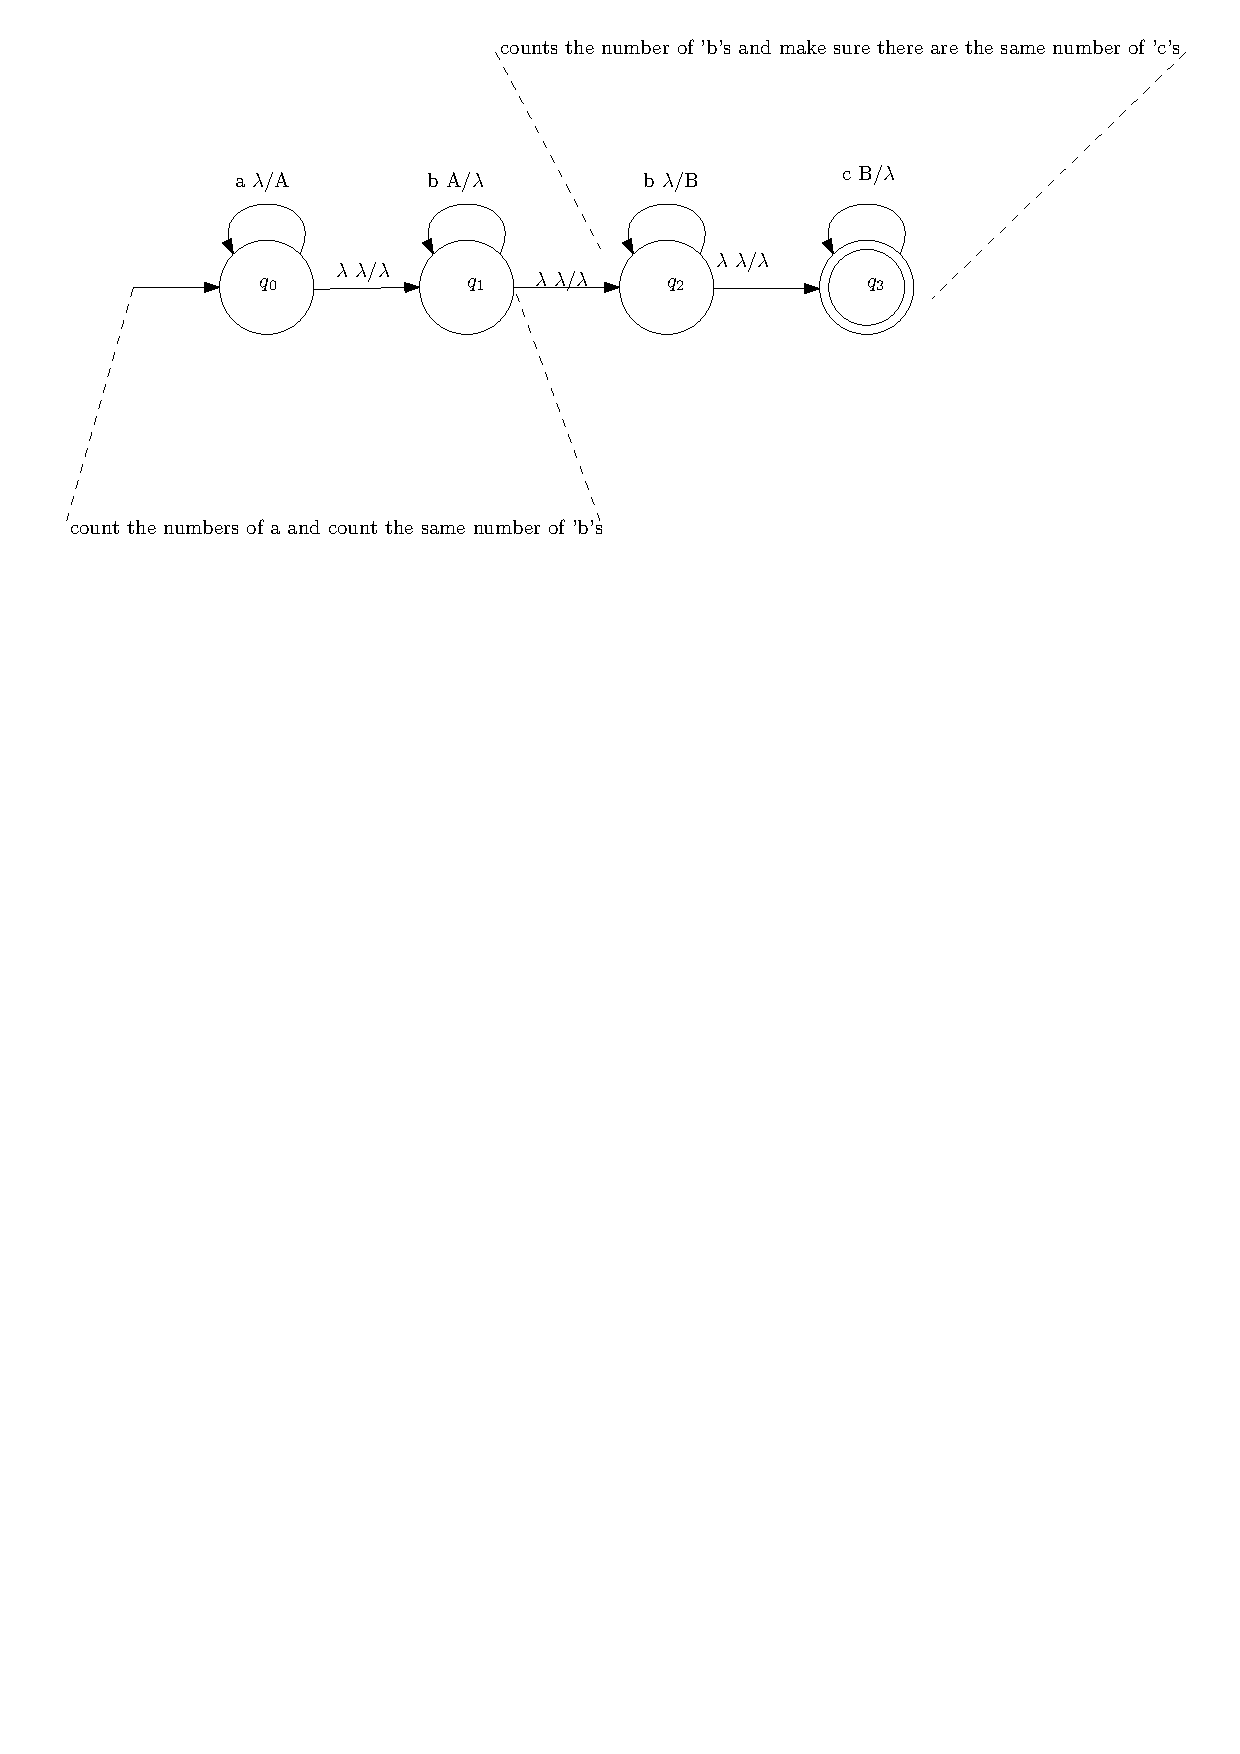
\includegraphics[width=0.75\textwidth]{PDA1.pdf}
\end{center}


The algorithm this PDA uses the fact that $j= i+k $ and turns $b^{j}$ to $b^{i+k}$ and then to $b^{i}b^{k}$ making $\{ a^i b^j c^k  \,|\, i,j,k \geq 0$ and $i + k = j \}$ in to $\{ a^i b^{i} b^{k} c^k  \,|\, i,k \geq 0\}$ so one now must only match the b to the number of 'a's and he nuber of 'c's.


{\bf 2.} {\em (25 points)} Let $M$ be the TM in Example 8.2.2 on page
261 (the machine for $a^i b^i c^i$ ).
Show the computation sequence for the strings $abc$ and $aabc$.

\begin{center}
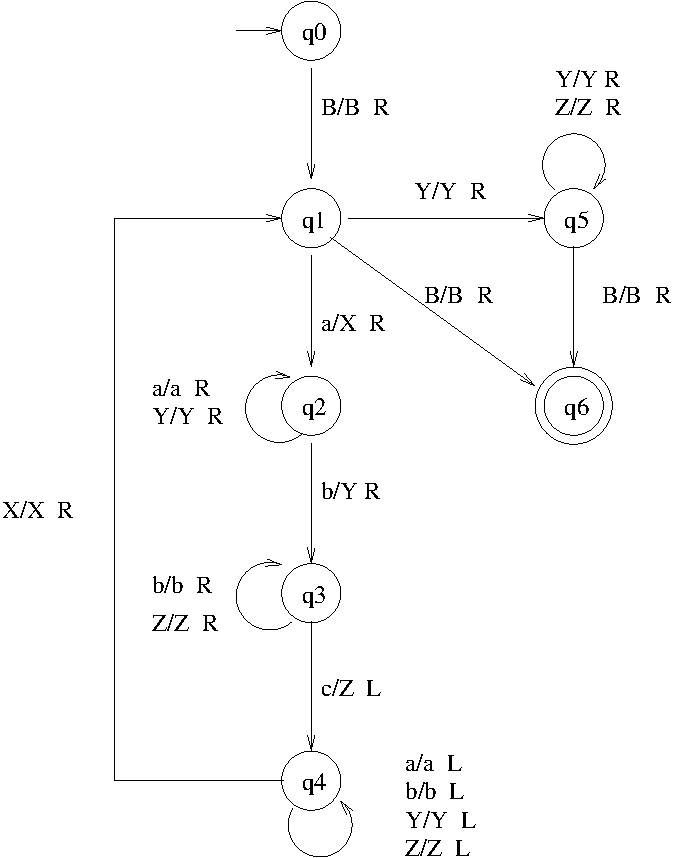
\includegraphics[width=0.50\textwidth]{example-8-2-2.pdf}
\end{center}

abc
\begin{itemize}
\item 
  \begin{tabular}{|c|c|c|c|c}
    \hline
    B&a&b&c&B\\
    \hline
    $\uparrow$&&&& 
  \end{tabular}
\item 
  \begin{tabular}{|c|c|c|c|c}
    \hline
    B&a&b&c&B\\
    \hline
    &$\uparrow$&&& 
  \end{tabular}
\item 
  \begin{tabular}{|c|c|c|c|c}
    \hline
    B&X&b&c&B\\
    \hline
    &&$\uparrow$&& 
  \end{tabular}
\item 
  \begin{tabular}{|c|c|c|c|c}
    \hline
    B&X&Y&c&B\\
    \hline
    &&&$\uparrow$& 
  \end{tabular}
  \item 
  \begin{tabular}{|c|c|c|c|c}
    \hline
    B&X&Y&Z&B\\
    \hline
    &&&&$\uparrow$
  \end{tabular}
      \item 
  \begin{tabular}{|c|c|c|c|c}
    \hline
    B&X&Y&Z&B\\
    \hline
   & $\uparrow$&&& 
  \end{tabular}  
\item
  \begin{tabular}{|c|c|c|c|c}
    \hline
    B&X&Y&Z&B\\
    \hline
&& $\uparrow$&& 
  \end{tabular}  
    \item 
  \begin{tabular}{|c|c|c|c|c}
    \hline
    B&X&Y&Z&B\\
    \hline
    &&& $\uparrow$& 
  \end{tabular}  
    \item 
  \begin{tabular}{|c|c|c|c|c}
    \hline
    B&X&Y&Z&B\\
    \hline
   &&&& $\uparrow$ 
  \end{tabular}  
\end{itemize}

aabc
\begin{itemize}
\item 
  \begin{tabular}{|c|c|c|c|c|c}
    \hline
    B&a&a&b&c&B\\
    \hline
    $\uparrow$&&&&&
  \end{tabular}
\item 
  \begin{tabular}{|c|c|c|c|c|c}
    \hline
    B&a&a&b&c&B\\
    \hline
     &$\uparrow$&&&&
  \end{tabular}
  \item 
  \begin{tabular}{|c|c|c|c|c|c}
    \hline
    B&X&a&b&c&B\\
    \hline
     &&$\uparrow$&&&
  \end{tabular}
  \item 
  \begin{tabular}{|c|c|c|c|c|c}
    \hline
    B&X&a&Y&c&B\\
    \hline
     &&&$\uparrow$&&
  \end{tabular}
  \item 
  \begin{tabular}{|c|c|c|c|c|c}
    \hline
    B&X&a&Y&Z&B\\
    \hline
    &&&&$\uparrow$&
  \end{tabular}
    \item 
  \begin{tabular}{|c|c|c|c|c|c}
    \hline
    B&X&a&Y&Z&B\\
    \hline
    &$\uparrow$&&&&
    
  \end{tabular}
\item 
  \begin{tabular}{|c|c|c|c|c|c}
    \hline
    B&X&a&Y&Z&B\\
    \hline
    &&$\uparrow$&&&
  \end{tabular}
\end{itemize}



\vspace{0.5in}
\hfill{{\em There are additional questions on the nextpage.}}

\newpage

{\bf 3.} {\em (20+5 points)}
Construct a TM that takes an input consisting of a sequence of
$a$'s followed by fewer or equal number of $b$'s; and outputs a string
where the number of $b$'s is the same as the original number of $a$'s. 

\begin{quote}
The input format is: $\{ a^i b^j \,|\, i,j \geq 0 \; \mbox{and} \;
                                         i \geq j \}$

The output format is: $\{ a^i b^i \,|\, i \geq 0 \}$

For example:\\
If the input is `$BaaaabbB$', the output should be `$BaaaabbbbB$'. \\
If the input is `$BaaabbbB$', the output should stay the same:
`$BaaabbbB$'.

\end{quote}

You may assume that the input will be in the desired format. There is no
need to check for errors.

Write the high-level algorithm executed by the machine and label the
sections {\em (5 points)}.
\begin{enumerate}
\item move right to the first a and replace it with A if it is not replace all A with a and all X with b
\item keep moving the right to the first b and or B and repalce it with a X
\item move to the left till A and repeat   
\end{enumerate}


\begin{center}
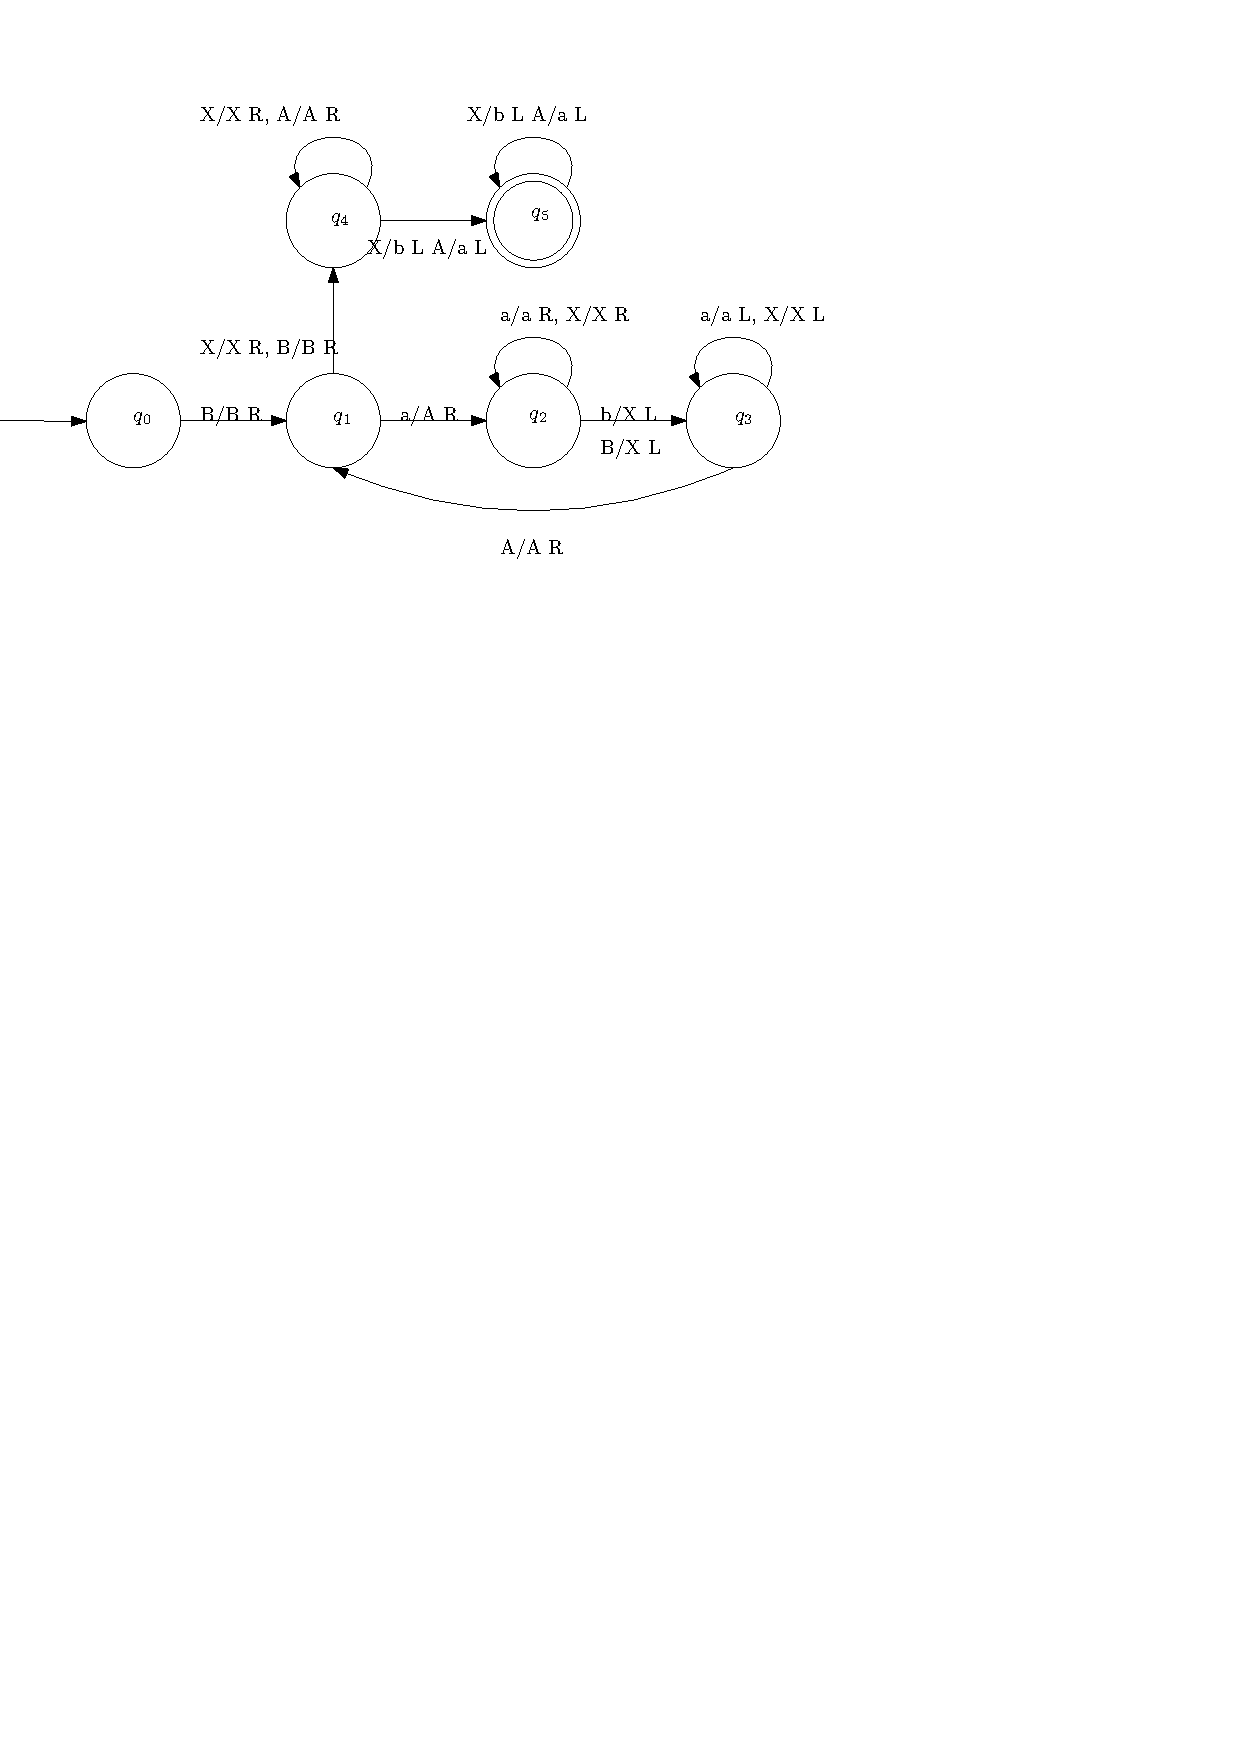
\includegraphics[width=0.75\textwidth]{TM1.pdf}
\end{center}


\vspace{0.2in}

{\bf 4.} {\em (20+5 points)}
Construct a TM that accepts the following language.\\
Write the high-level algorithm executed by the machine and label the
sections {\em (5 points)}.

$\{ a^i b^j c^k  \,|\, i + j = k\}$


\begin{enumerate}
\item move right to a mark A move to the first c and mark it C
\item move left to the first A or X  move rigth if a mark A if b mark X if C got to aceept
\item check if there are any unmaked cells
\end{enumerate}

\begin{center}
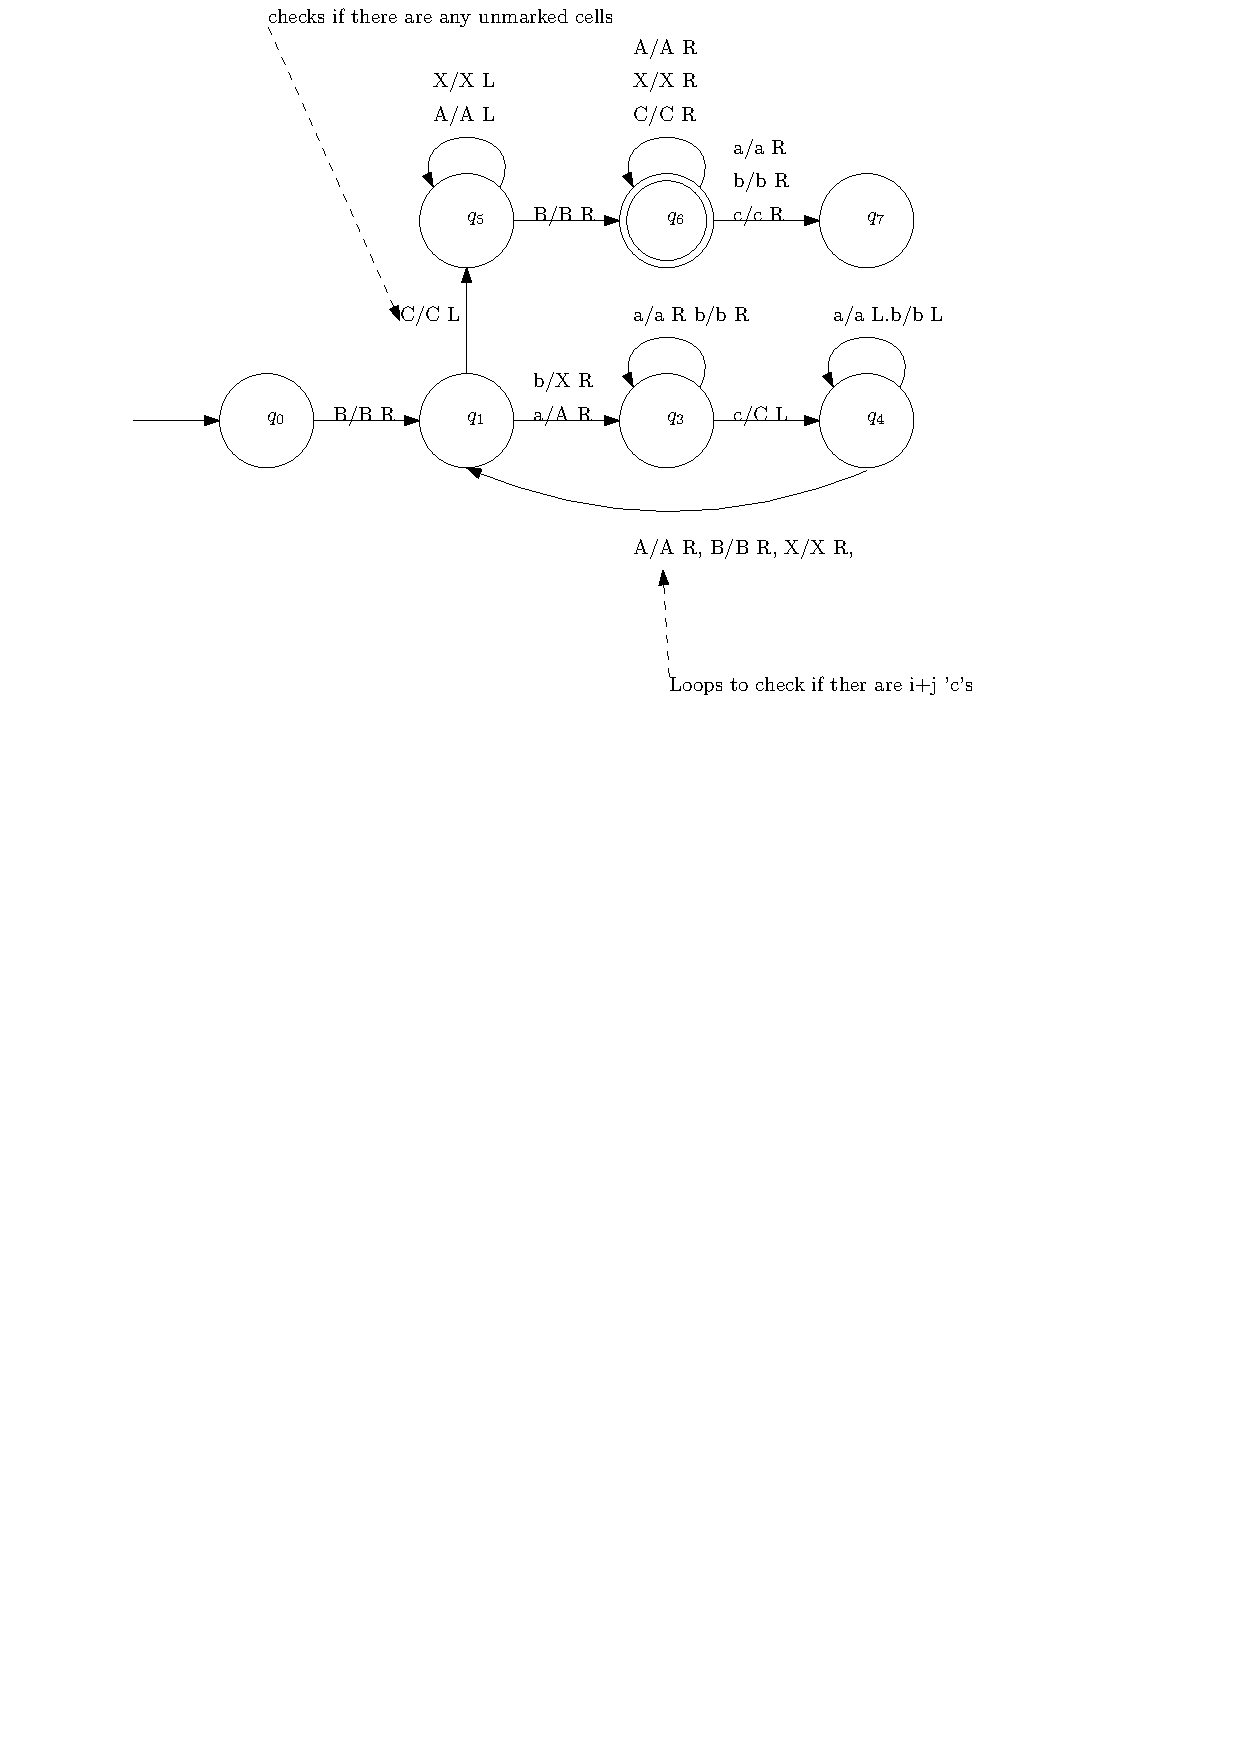
\includegraphics[width=0.75\textwidth]{TM2.pdf}
\end{center}


\end{document}

